\chapter{Implementação}

Neste capítulo, a solução é  transformada num sistema funcional com até certa limitação, e as regras, princípios e tecnologias estabelecidas são testadas. O que diz respeito aos resultados observados são listados juntos à parâmetros relevantes.

\section{Ambiente de Desenvolvimento}
O ambiente de desenvolvimento foi estruturado utilizando o VS Code como principal editor de código, com a execução da aplicação ocorrendo de maneira local (localhost) durante esta etapa do projeto. O controle de versão se deu por meio do git e github. A organização do repositório seguiu uma estrutura modular para otimizar o gerenciamento dos arquivos, destacando-se a definição e a exportação padronizada dos componentes em React, o que garantiu a modularidade, a reutilização eficiente do código e a clareza na construção da interface web enquanto a outra divisão interna dispõe de poucos scripts.

\section{Estrutura da Aplicação}
\begin{figure}[H]
	\caption{\label{fig_pack}Diagrama de Pacotes}
	\begin{center}
	    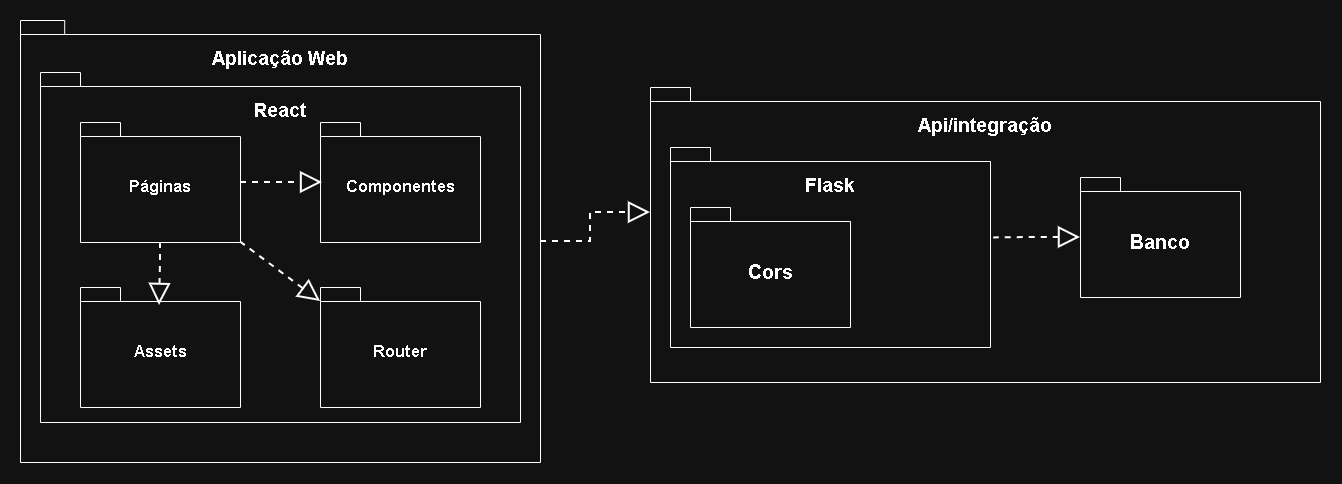
\includegraphics[scale=0.3]{imagens/diag_pack.png}
	\end{center}
\end{figure}

\section{Implementação dos Componentes}
No sistema propriamente dito, os componentes definidos no modelo conceitual foram aplicados objetivamente, considerando que não há a exata possibilidade de replicar o descrito, e também boas práticas e que melhores arranjos poderem ser usados. Nesse sentido, as funcionalidades previstas se encontram majoritariamente no pacote Web, como gerenciamento, visualização, relatórios e em menor quantidade nos demais como na filtragem e edição de registros.

\section{Integração dos Módulos}
\begin{figure}[H]
	\caption{\label{fig_implant}Diagrama de Implantação}
	\begin{center}
	    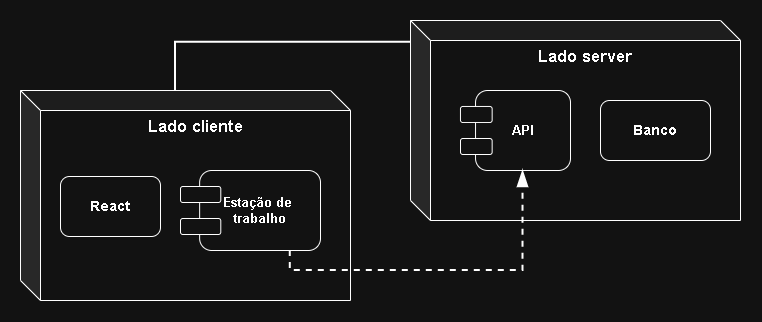
\includegraphics[scale=0.6]{imagens/diag_implant.png}
	\end{center}
\end{figure}

\section{Testes Realizados}
Os tipos de testes que serão utilizados são relacionados principalmente ao funcionamento de cada unidade modular, usabilidade e aceitação do usuário. Porém, para esta versão, testes ainda estão para ser realizados.

\section{Resultados Obtidos}
O resultado, até pelo menos a primeira versão desenvolvida e apresentada, foi um sistema plenamente funcional. A integração entres os componentes em nível de arquitetura funciona sem erros, provindo persistência dos dados, realização de CRUD, como também consistência. E do mesmo modo, as interfaces de usuário possibilitam as operações esperadas.

\section{Limitações da Implementação}
Alguns problemas menores e limitações são testemunhados quanto a certas tecnologias e recursos utilizados. A que se apresenta mais relevante é a limitação do próprio banco de dados escolhido, que para a finalidade do sistema é o suficiente, mas que pode vir a ser um problema seja necessário escalar progressivamente a solução. Há também a própria dinâmica do React que não possibilita uma comunicação mais fluida entre componentes e a manutenção de versões das bibliotecas Python.